\documentclass{article}
\usepackage[margin=1in]{geometry}
\usepackage{physics}
\usepackage{graphicx}
\usepackage{caption}
\usepackage{amsmath}
\usepackage{bm}
\usepackage{authblk}
\usepackage{empheq}
\usepackage{amsfonts}
\usepackage{esint}
\usepackage[makeroom]{cancel}
\usepackage{dsfont}
\usepackage{centernot}
\usepackage{mathtools}
\usepackage{bigints}
\usepackage{amsthm}
\theoremstyle{definition}
\newtheorem{defn}{Definition}[section]
\newtheorem{prop}{Proposition}[section]
\newtheorem{rmk}{Remark}[section]
\newtheorem{thm}{Theorem}[section]
\newtheorem{exmp}{Example}[section]
\newtheorem{prob}{Problem}[section]
\newtheorem{sln}{Solution}[section]
\newtheorem*{prob*}{Problem}
\newtheorem{exer}{Exercise}[section]
\newtheorem*{exer*}{Exercise}
\newtheorem*{sln*}{Solution}
\usepackage{empheq}
\usepackage{hyperref}
\usepackage{tensor}
\usepackage{xcolor}
\hypersetup{
	colorlinks,
	linkcolor={black!50!black},
	citecolor={blue!50!black},
	urlcolor={blue!80!black}
}


\newcommand*\widefbox[1]{\fbox{\hspace{2em}#1\hspace{2em}}}

\newcommand{\p}{\partial}
\newcommand{\R}{\mathbb{R}}
\newcommand{\C}{\mathbb{C}}
\newcommand{\lag}{\mathcal{L}}
\newcommand{\nn}{\nonumber}
\newcommand{\ham}{\mathcal{H}}
\newcommand{\M}{\mathcal{M}}
\newcommand{\I}{\mathcal{I}}
\newcommand{\K}{\mathcal{K}}
\newcommand{\F}{\mathcal{F}}
\newcommand{\w}{\omega}
\newcommand{\lam}{\lambda}
\newcommand{\al}{\alpha}
\newcommand{\be}{\beta}
\newcommand{\x}{\xi}

\newcommand{\G}{\mathcal{G}}

\newcommand{\f}[2]{\frac{#1}{#2}}

\newcommand{\ift}{\infty}

\newcommand{\lp}{\left(}
\newcommand{\rp}{\right)}

\newcommand{\lb}{\left[}
\newcommand{\rb}{\right]}

\newcommand{\lc}{\left\{}
\newcommand{\rc}{\right\}}


\newcommand{\V}{\mathbf{V}}
\newcommand{\U}{\mathcal{U}}
\newcommand{\Id}{\mathcal{I}}
\newcommand{\D}{\mathcal{D}}
\newcommand{\Z}{\mathcal{Z}}

%\setcounter{chapter}{-1}


%\makeatletter
%\renewcommand{\@chapapp}{Part}
%\renewcommand\thechapter{$\bf{\ket{\arabic{chapter}}}$}
%\renewcommand\thesection{$\bf{\ket{\arabic{section}}}$}
%\renewcommand\thesubsection{$\bf{\ket{\arabic{subsection}}}$}
%\renewcommand\thesubsubsection{$\bf{\ket{\arabic{subsubsection}}}$}
%\makeatother



\usepackage{subfig}
\usepackage{listings}
\captionsetup[lstlisting]{margin=0cm,format=hang,font=small,format=plain,labelfont={bf,up},textfont={it}}
\renewcommand*{\lstlistingname}{Code \textcolor{violet}{\textsl{Mathematica}}}
\definecolor{gris245}{RGB}{245,245,245}
\definecolor{olive}{RGB}{50,140,50}
\definecolor{brun}{RGB}{175,100,80}
\lstset{
	tabsize=4,
	frame=single,
	language=mathematica,
	basicstyle=\scriptsize\ttfamily,
	keywordstyle=\color{black},
	backgroundcolor=\color{gris245},
	commentstyle=\color{gray},
	showstringspaces=false,
	emph={
		r1,
		r2,
		epsilon,epsilon_,
		Newton,Newton_
	},emphstyle={\color{olive}},
	emph={[2]
		L,
		CouleurCourbe,
		PotentielEffectif,
		IdCourbe,
		Courbe
	},emphstyle={[2]\color{blue}},
	emph={[3]r,r_,n,n_},emphstyle={[3]\color{magenta}}
}


\begin{document}
\begin{center}
	\huge{Questions/Ideas \#2 (\textit{to be continued})}\\
	$\,$\\
	\normalsize{\today}\\
	\normalsize{Huan Bui}
\end{center}

Hi Evan, here's a layout of this document:
\begin{itemize}
	\item Part 1 focuses on the change of coordinates $\xi \to \phi(x^\mu)$ and its Jacobian. I will consider only the integral over $\mathbb{R}^2$ and will try to discuss a few things about the $\mathbb{R}^d$ integral. Here's a summary of this part: 
	\begin{enumerate}
		\item For a given $E$ such that $P(t^E s) = tP(s)$, we can't in general have a coordinate transformation $\xi \to \phi(t^\mu)$ such that $\abs{\det J(\phi)} = \text{C}\times t^{\dots}$ where $C$ is a constant that is only dependent on the dimension $n$ of $\mathbb{R}^n$. I will show this for the $n=2$ case, but we can see it is even more difficult to make $\abs{J(\phi)}$ independent of angles when $n>2$.  
		
		\item I then consider the transformation $\xi \to t^E s$ such that $P(t^E s) = tP(s) = t$. This raises some concerns about the bijectivity of $\phi$ but makes the integral much easier to handle. I will consider the $n=4$, $E = \text{diag}(1/2,1/4)$ case and see what I can generalize from there.
		
		\item I consider the integral 
		\begin{align}
		\int_{\mathbb{R}^d}e^{iP(\xi) - i x\cdot \xi}\,d\xi.
		\end{align}
	\end{enumerate}

	
	\item  In Part 2, I consider some oscillatory integrals and in what sense they converge.  
\end{itemize}
	
\hrule

\begin{enumerate}
	\item The integral over $\mathbb{R}^2$ we went over on Friday, Nov 8 has the form
	\begin{align}
	I \equiv \int_{\mathbb{R}^2}f(\xi)\,d\xi_1d\xi_2.
	\end{align}
	Let $E = \text{diag}(1/d_1, 1/d_2)$, which corresponds to $P(\xi) = \xi_1^{d_1} + \xi_2^{d_2}$. Suppose all $d_i$'s are even, and that $1/d_1 \geq 1/d_2$. On Friday, we considered the transformation
	\begin{align}
	\xi \to \phi(t,\theta) \equiv t^Es  = t^E\begin{bmatrix}
	\cos\theta \\ \sin\theta
	\end{bmatrix} = \begin{bmatrix}
	t^{1/d_1} \cos\theta \\ t^{1/d_2}\sin\theta
	\end{bmatrix}.
	\end{align}
	The Jacobian of this transformation is
	\begin{align}
	J = \det\begin{bmatrix}
	\f{{t^{-1+1/d_1}} \cos \theta}{d_1} & -t^{1/d_1} \sin
	\theta  \\
	\f{{t^{-1+1/d_2}-} \sin \theta }{d_2} & t^{1/d_2} \cos
	\theta  \\
	\end{bmatrix} = t^{\tr E-1}\lp\frac{d_1\sin ^2\theta + d_2\cos^2\theta}{d_1 d_2}\rp.
	\end{align}
	We can consider two cases $d_1 = d_2$ and $d_1 \neq d_2$
	\begin{enumerate}
		\item \textbf{\textit{Case 1:}} If $d_1 = d_2 = d$ then 
		\begin{align}
		J = \f{t^{-1+2/d}}{d^2} = \f{t^{\tr E -1 }}{d^2}.
		\end{align}
		We have discussed how $\phi: (0,\infty)\times [0,2\pi] \to \mathbb{R}^2$ is bijective. So the original integrals becomes 
		\begin{align}
		I &= \int_{\mathbb{R}^2}f(\xi)\,d\xi_1d\xi_2 \nn\\
		&= \int_0^\infty \int_0^{2\pi} f(t^Es) \abs{J}\,dtd\theta\nn\\
		&= \int_0^\infty \int_0^{2\pi}f\begin{bmatrix}
		t^{1/d} \cos\theta \\ t^{1/d}\sin\theta
		\end{bmatrix}\cdot\lp \f{t^{\tr E -1 }}{d^2} \rp\,dtd\theta.
		\end{align}
		When $f(\xi) = e^{iP(\xi)} \to e^{iP(t^Es)} = e^{itP(s)}$ we have
		\begin{align}
		{I = \f{1}{d^2}\int_0^\infty \int_0^{2\pi} t^{\tr E -1 } e^{it(\cos^d\theta + \sin^d \theta)}\,dtd\theta}
		\end{align}
		
		
		\begin{enumerate}
			\item \textit{Case 1.1:} When $d=2$, $\tr E = 1$, and so 
			\begin{align}
			I = 2\pi \int^\infty_0 e^{it}\,dt.
			\end{align}
			This integral diverges (which I could see upon differentiating under the integral sign). So, I interpret this as a Fourier transform (up to factors of $2\pi$) of the step function
			\begin{align}
			g(x) = \begin{cases}
			1 \quad x\geq 0 \\ 
			0 \quad x < 0
			\end{cases}
			\end{align}
			evaluated at $\omega=1$, because
			\begin{align}
			\F[g](\omega)\bigg\vert_1 \propto \int_{-\infty}^{\infty} g(t)e^{i\cdot 1 \cdot 1}\,dt &= \underbrace{\int^0_{-\infty}g(t)e^{it}\,dt}_0 + \int^\infty_0 g(t)\cdot e^{it}\,dt = \int^\infty_0 e^{it}\,dt.
			\end{align}
			I can also interpret $I$ as a Laplace transform of some other function, but I don't think we gain anything from doing that.\\
			
			
			\item \textit{Case 1.2:} When $d = 2m >2$ then the original integral becomes
			\begin{align}
			I = \f{1}{(2m)^2}\int_0^\infty \int_0^{2\pi} t^{\tr E -1 } e^{it(\cos^{2m}\theta + \sin^{2m} \theta)}\,dtd\theta.
			\end{align}
			Base on a number of tests in Mathematica I think these integrals converge, but I can't seem to deduce any pattern. For example:
			\begin{align}
			&d=4: I = \f{2 + 2i}{16} \sqrt{2\pi}\, K\lb \f{1}{2} \rb\nn\\
			&d=6: I = \f{(2 \pi^2)\,_2F_1\lb \f{1}{6}, \f{2}{3}, 1, \f{9}{25}\rb (-3.50882 - 2.02582 i)}{36\Gamma\lb \f{-1}{3} \rb}\nn\\
			&d=8: I = \f{1}{2} \sqrt[8]{-1}\, \Gamma\lb \f{9}{8} \rb^2\nn\\
			&d=10: \dots\nn
			\end{align}
			
			
		\end{enumerate}
			
			
			
			
			
			
			
		\item \textbf{\textit{Case 2:}} If $1/d_1 > 1/d_2$ and both $d_1,d_2$ are even, then the Jacobian
		\begin{align}
		J = t^{\tr E - 1}\lp \f{d_1\sin^2\theta + d_2 \cos^2\theta}{d_1d_2} \rp
		\end{align}
		is always dependent on $\theta$. Thus, the parameterization 
		\begin{align}
		\phi(t,\theta) = t^E\begin{bmatrix}
		\cos\theta \\ \sin\theta
		\end{bmatrix}
		\end{align}
		now becomes disadvantageous because the integral $I$ now contains $t$ and $\theta$ in both the exponent and scaling factor $\abs{J(\phi)}$. I think this requires us to consider a new parameterization
		\begin{align}
		\Phi(t,\theta) = t^E s(\theta)
		\end{align}
		where $P[s(\theta)] = 1$. This does not guarantee the angle-independence of the volume element, but we can always integrate out the angles separately. 
		
		\begin{enumerate}		
		\item \textit{Case 1:} Consider for example $d_1 = 2, d_2 = 4$. With this, $P(\xi) = \xi_1^2 + \xi_2^4$,
		and we know very well $E = \text{diag}(1/2, 1/4)$. We can consider the parameterization $\Phi:(0,\infty)\times [0,\pi]\to \mathbb{R}^2$
		\begin{align}
		\Phi(t,\theta) = \begin{cases}
		t^E\begin{bmatrix}
		\sin (2\theta) &\,\,\,\,& \sqrt{\cos (2\theta)}
		\end{bmatrix}^\top \quad t\in (0,\infty), \theta \in [0,\pi/4)\\
		t^E\begin{bmatrix}
		\sin (2\theta) & -\sqrt{-\cos (2\theta)}
		\end{bmatrix}^\top \quad t\in (0,\infty), \theta \in [\pi/4,3\pi/4]\\
		t^E\begin{bmatrix}
		\sin (2\theta) &\,\,\,\,& \sqrt{\cos (2\theta)}
		\end{bmatrix}^\top \quad t\in (0,\infty), \theta \in (3\pi/4,\pi]
		\end{cases}.
		\end{align}
		\begin{figure}[!htb]
			\centering
			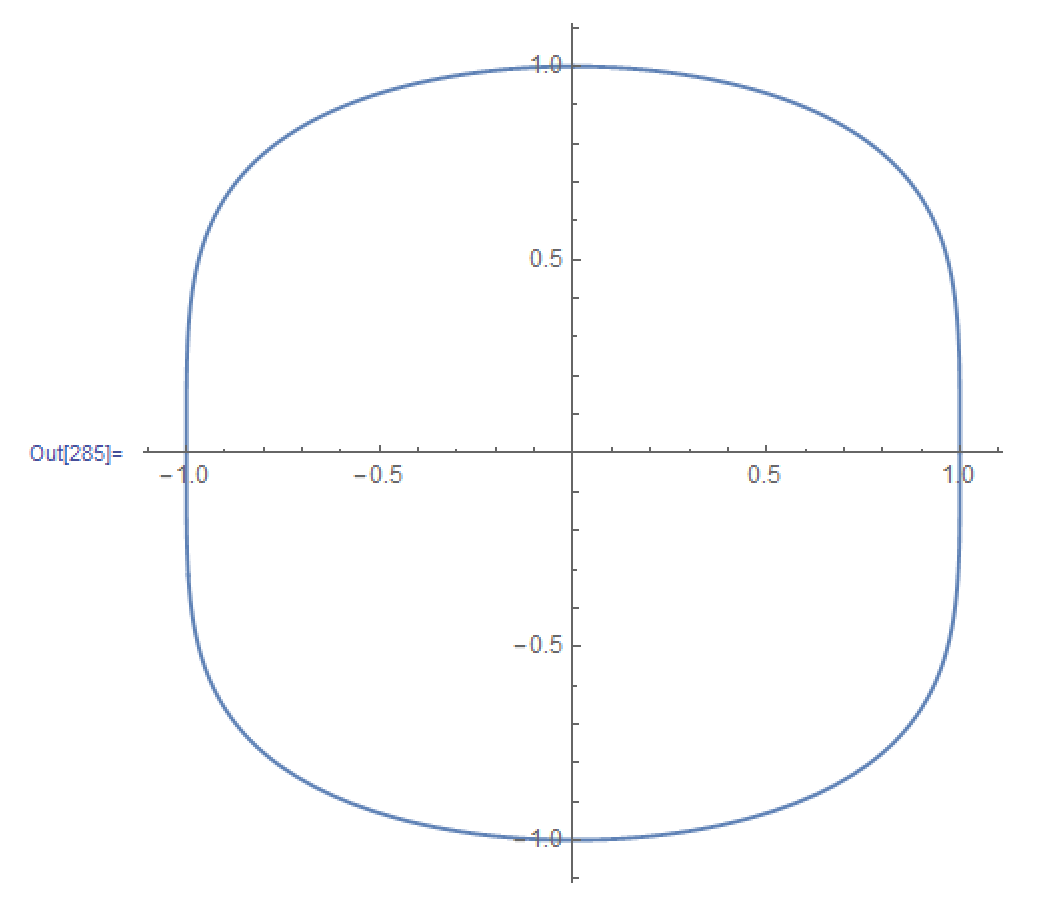
\includegraphics[scale=0.3]{param}
			\caption{$\Phi(1,\theta)$, for $\theta \in [0,\pi]$.}
		\end{figure}\\
	
		We see that 
		\begin{align}
		P(\xi)\to P(t^Es) = tP(s) = t\lb \sin^2(2\theta) + \lp\pm \sqrt{\pm \cos(2\theta)}\rp^4  \rb = t.
		\end{align}
		With this, the original integral becomes 
		\begin{align}
		I = \int^\infty_0 \int^{\pi/4}_0 e^{it}\abs{J(\Phi)}\,dtd\theta + \int^\infty_0\int^{3\pi/4}_{\pi/4}e^{it}\abs{J(\Phi)}\,dtd\theta + \int^\infty_0 \int^{\pi}_{3\pi/4}e^{it}\abs{J(\Phi)}\,dtd\theta. 
		\end{align}
		Next we find what $\abs{J(\Phi)}$ is for each integral. We consider two cases: $t^E(\sin(2\theta),\sqrt{\cos(2\theta)})^\top$ and $t^E(\sin(2\theta), -\sqrt{-\cos(2\theta)})^\top$. \\
		
		When $\theta\in [0,\pi/4) \cup (3\pi/4,\pi]$, we have
		\begin{align}
		\abs{J(\Phi)} 
		= 
		\abs{\det\begin{bmatrix}
		\frac{\sin (2 \theta )}{2 \sqrt{t}} & 2 \sqrt{t} \cos (2 \theta ) \\
		\frac{\sqrt{\cos (2 \theta )}}{4 t^{3/4}} & -\frac{\sqrt[4]{t} \sin (2 \theta )}{\sqrt{\cos (2\theta )}} 
		\end{bmatrix}} = \frac{1}{2 \sqrt[4]{t} \sqrt{\cos (2 \theta )}}
		\end{align}
		We should check if the $\theta$ integrals converge in these cases (they do):
		\begin{align}
		\int^{\pi/4}_0 \f{1}{\sqrt{\cos(2\theta)}}\,d\theta = \int^{3\pi/4}_{\pi/4} \f{1}{\sqrt{\cos(2\theta)}}\,d\theta = \frac{K\left(\frac{1}{2}\right)}{\sqrt{2}}.
		\end{align}
		When $\theta \in [\pi/4,3\pi/4]$, we have
		\begin{align}
		\abs{J(\Phi)} =\abs{\det\begin{bmatrix}
			\frac{\sin (2 \theta )}{2 \sqrt{t}} & 2 \sqrt{t} \cos (2 \theta ) \\
			-\frac{\sqrt{-\cos (2 \theta )}}{4 t^{3/4}} & -\frac{\sqrt[4]{t} \sin (2 \theta )}{\sqrt{-\cos
					(2 \theta )}} 
			\end{bmatrix}} = \frac{1}{2 \sqrt[4]{t} \sqrt{-\cos (2 \theta )}}.
		\end{align}
		We check if the $\theta$ integral converges in this case (it does):
		\begin{align}
		\int^{3\pi/4}_{\pi/4}\f{1}{\sqrt{-\cos(2\theta)}}\,d\theta = -i \left(\sqrt{2} K\left(\frac{1}{2}\right)-2 K(2)\right).
		\end{align}
		Thus, it is possible to integrate out all the angle elements to find 
		\begin{align}
		I = \Omega\int^\infty_0 t^{\tr E- 1 }e^{it}\,dt=  \Omega\int^\infty_0 t^{-1/4}e^{it}\,dt. 
		\end{align}
		where $\Omega$ is constant. \\
		
		At this point, we can use van der Corput's lemma to show $I$ is bounded. We can also evaluate this directly in Mathematica to find
		\begin{align}
		I = \Omega (-1)^{3/8} \Gamma \left(\frac{3}{4}\right).
		\end{align}
		
		
		\item In general... (\textit{to be continued})
		
		
		
		\item What happens when we look at the integral
		\begin{align}
		I(x) = \int_{\mathbb{R}^d}e^{iP(\xi) - ix\cdot \xi}\,d\xi = \int^\infty_0\int_{\mathcal{S}}e^{iP(t^Es) - ix\cdot t^E s}\,d\xi = \int^\infty_0\int_{\mathcal{S}}e^{it - ix\cdot t^E s}\,d\xi
		\end{align}
		where $P(s) = 1$? One strategy is to expand the $x\cdot t^E s$ term and see what dominates
		\begin{align}
		I(x) = \sum_{n=0}^\infty\int^\infty_0\int_{\mathcal{S}}e^{it}\f{\lp-ix\cdot t^Es\rp^n}{n!}\,d\xi.
		\end{align}
		Is there a way to get some kind of bounds for each term in the sum? When $x=0$, $x \ll 1$, etc. or when $s\in \mathcal{S}$, what can we say about high-$n$ terms in the expansion of $I(x)$?   
		
		\end{enumerate}
		
	\end{enumerate}



	\item Some oscillatory integral stuff...

\end{enumerate}
	
	
	

	
\end{document}